% ============================================================================
% SMART -- 3-slide talk deck. TikZ-driven visual flow, Beamer.
% Slide 1: motivation + bio-informed MoR pipeline (TikZ).
% Slide 2: results -- performance / params / tokens / honest negatives (TikZ).
% Slide 3: why token reduction is biologically meaningful + directions (TikZ).
% Compile from paper/:  latexmk -pdf slides_smart.tex
% ============================================================================
\documentclass[aspectratio=169,11pt]{beamer}
\usetheme{Madrid}
\usecolortheme{seahorse}
\usepackage{booktabs}
\usepackage{colortbl}
\usepackage{tikz}
\usepackage{fontawesome5}
\usetikzlibrary{arrows.meta,positioning,fit,backgrounds,calc,shapes.geometric}
\usepackage{amsmath}
% Nature-style light palette for table cell/row shading (soft, desaturated).
\definecolor{natgood}{HTML}{DCEDD3}   % soft green -- good / peak
\definecolor{natbad}{HTML}{FAD9D6}    % soft red   -- collapse / poor
\definecolor{nathead}{HTML}{E8EEF5}   % soft blue-gray -- header
\definecolor{natcost}{HTML}{FBE7D6}   % soft orange -- rising compute cost

\definecolor{accentA}{RGB}{0,120,90}     % biology / markers (green)
\definecolor{accentB}{RGB}{190,80,20}    % recursion / compute (orange)
\definecolor{neg}{RGB}{155,20,45}        % negatives (red)
\definecolor{panelA}{RGB}{232,245,240}
\definecolor{panelB}{RGB}{250,240,230}
\colorlet{subcap}{gray!60!black}

\setbeamercolor{frametitle}{bg=accentA,fg=white}
\setbeamercolor{title}{fg=accentA}
\setbeamertemplate{navigation symbols}{}
\setbeamerfont{frametitle}{size=\large}

\newcommand{\good}[1]{\textcolor{accentA}{\textbf{#1}}}
\newcommand{\bad}[1]{\textcolor{neg}{\textbf{#1}}}
\newcommand{\comp}[1]{\textcolor{accentB}{\textbf{#1}}}

% shared node styles (adapted from the paper's system-overview TikZ)
\tikzset{
  stage/.style={rounded corners=3pt, draw=black!30, fill=white, line width=0.7pt,
                minimum height=11mm, text width=19mm, align=center, font=\scriptsize},
  flow/.style={-{Stealth[length=2.2mm]}, line width=1pt, draw=accentB},
  bioflow/.style={-{Stealth[length=2.4mm]}, line width=1.1pt, draw=accentA, dashed},
  lbl/.style={font=\tiny, text=subcap},
}

\title[SMART]{\textbf{SMART}: Biology-Informed Mixture-of-Recursions}
\subtitle{Token reduction + adaptive recursion for genomic classification}
\author[Howlader et al.]{Howlader \and Roy \and Islam \and Le}
\institute[ISU \textbullet\ Stanford]{\faUniversity~Iowa State University \quad\textbullet\quad \faUniversity~Stanford University}
\date{}

\begin{document}

% ======================= SLIDE 1: motivation + design ======================
\begin{frame}[shrink=15]{Problem \& design: a biology-informed recursive transformer}
\begin{block}{\footnotesize Problem statement}
\scriptsize
Classify a cell/sample from $x\!\in\!\mathbb{R}^{N}$ ($N\!\approx\!20$k genes) \emph{accurately \& cheaply}. Two costs are our targets:
\good{(T) token cost} --- attention is $\mathbf{O(N^2)}$ in genes; \quad \comp{(F) FLOP/depth cost} --- a $K$-layer stack is $\mathbf{O(K)}$ FLOPs \emph{and} $O(K)$ params, spent uniformly on every token.
\textbf{Goal:} \good{(T) $O(N^2)\!\to\!O(M^2)$}, $M\!\ll\!N$; \;\comp{(F) $O(K)\!\to$ adaptive per-token depth} at \good{constant params} --- guided by biology.
\end{block}
\centering
\resizebox{0.74\textwidth}{!}{%
\begin{tikzpicture}[node distance=6.5mm]
  % ---- top row: marker selection (token reduction) ----
  \node[stage, fill=panelA] (inp) {{\textcolor{accentA}{\faDna}}\\[1pt]\textbf{Expression}\\[1pt]{\tiny\textcolor{subcap}{$x\!\in\!\mathbb{R}^{N\approx 20k}$}}};
  \node[stage, right=of inp, fill=panelA] (router) {{\textcolor{accentA}{\faSearch}}\\[1pt]\textbf{Marker Router}\\[1pt]{\tiny\textcolor{subcap}{$M$ query slots}}};
  \node[stage, right=of router, fill=panelA] (mtok) {{\textcolor{accentA}{\faTags}}\\[1pt]\textbf{$M$ Marker Tokens}\\[1pt]{\tiny\textcolor{subcap}{$O(M^2)\!\ll\!O(N^2)$}}};
  % ---- bottom row: recursion + routing ----
  \node[stage, below=15mm of inp, fill=panelB] (shared) {{\textcolor{accentB}{\faRedo}}\\[1pt]\textbf{Shared Block}\\[1pt]{\tiny\textcolor{subcap}{$f_\theta\times K$, one copy}}};
  \node[stage, right=of shared, fill=panelB] (mor) {{\textcolor{accentB}{\faFilter}}\\[1pt]\textbf{MoR Depth Router}\\[1pt]{\tiny\textcolor{subcap}{funnel; adaptive $d_m$}}};
  \node[stage, right=of mor, fill=panelB] (pool) {{\textcolor{accentB}{\faCompress}}\\[1pt]\textbf{Mean-pool}};
  \node[stage, right=of pool, fill=panelB] (clf) {{\textcolor{accentB}{\faChartBar}}\\[1pt]\textbf{Phenotype}\\[1pt]{\tiny\textcolor{subcap}{cell type / cancer}}};
  % ---- biological prior node ----
  \node[stage, right=of mtok, draw=accentA, line width=1.2pt, fill=panelA, text width=22mm]
        (gint) {{\textcolor{accentA}{\faProjectDiagram}}\\[1pt]\textbf{Gene / Pathway Graph}\\[1pt]{\tiny\textcolor{subcap}{co-expr.\,/\,Reactome $\pi$ (label-free)}}};

  \draw[flow, draw=accentA] (inp) -- (router);
  \draw[flow, draw=accentA] (router) -- (mtok);
  \draw[flow] (shared) -- (mor);
  \draw[flow] (mor) -- (pool);
  \draw[flow] (pool) -- (clf);
  % tokens drop down into the recursion
  \draw[flow] (mtok.south) -- ++(0,-4mm) -| (shared.north);
  % weight-shared loop
  \draw[{Stealth[length=2.2mm]}-, line width=1pt, draw=accentB]
        (shared.south west) .. controls ++(0,-6mm) and ++(0,-6mm) .. (shared.south east)
        node[midway, below, font=\tiny, text=accentB]{$\times K$ weight-shared};
  % biology prior injected into router (centerpiece)
  \draw[bioflow] (gint.south) -- ++(0,-8mm) -| (mor.north)
        node[pos=0.75, above, font=\tiny, text=accentA]{$+\,\beta_t\pi_m$};

  \begin{scope}[on background layer]
    \node[rounded corners=5pt, fill=panelA, fit=(inp)(gint)] {};
    \node[rounded corners=5pt, fill=panelB, fit=(shared)(clf)] {};
  \end{scope}
\end{tikzpicture}}

\vspace{1mm}
{\scriptsize \good{A}\;marker selection: $N\!\to\!M$ tokens, $O(M^2)$ attention \quad\textbullet\quad \comp{B}\;one shared block $\times K$ + \comp{MoR} adaptive depth \quad\textbullet\quad \good{prior} $\pi$ nudges \good{hubs} deeper (label-free)}
\end{frame}

% ======================= SLIDE 2: results ==================================
\begin{frame}{Results: efficiency wins, accuracy is a wash (honest negatives)}
\begin{columns}[T]
\column{0.5\textwidth}
\centering\textbf{\footnotesize Token reduction}\\[-1mm]
{\scriptsize macro-F1 vs \# marker tokens $M$}\\[1mm]
\resizebox{\linewidth}{!}{%
\begin{tabular}{lcccc}
\toprule
\rowcolor{nathead}
 & $M{=}16$ & $M{=}64$ & $M{=}128$ & $M{=}256$ \\
\midrule
Tabula Muris & 35.4 & 64.6 & 71.3 & \cellcolor{natgood}75.3 \\
Prototype    & 62.5 & 90.2 & 94.8 & \cellcolor{natgood}97.2 \\
Pancreas     & 43.9 & 53.0 & 58.4 & \cellcolor{natgood}57.7 \\
Prostate     & 74.1 & 78.5 & 77.0 & \cellcolor{natgood}78.2 \\
\bottomrule
\end{tabular}}
\vspace{2mm}

\centering\textbf{\footnotesize Vanilla vs Recursive vs MoR @ $K^\star{=}4$}\\[1mm]
\resizebox{\linewidth}{!}{%
\begin{tabular}{lrrr}
\toprule
\rowcolor{nathead}
pancreas & Vanilla & Recursive & MoR \\
\midrule
Params (unique) & 299{,}136 & \cellcolor{natgood}74{,}784 & \cellcolor{natgood}75{,}168 \\
FLOPs/sample    & 62.9\,M & 62.9\,M & \cellcolor{natgood}38.9\,M \\
Compute saved   & --- & --- & \cellcolor{natgood}38\% \\
macro-F1        & 54.1$\pm$0.8 & 57.3$\pm$5.8 & 54.2$\pm$0.9 \\
accuracy        & 92.4 & 91.8 & 91.1 \\
\bottomrule
\end{tabular}}\\[1mm]
{\tiny Equal accuracy: MoR $=$ \good{4$\times$ fewer params} than Vanilla $+$ \comp{38\% fewer FLOPs} than Recursive.}

\column{0.5\textwidth}
% TikZ compute-funnel: the one decisive positive
\centering\textbf{\footnotesize Adaptive depth $\Rightarrow$ compute funnel}\\[1mm]
\resizebox{0.92\linewidth}{!}{%
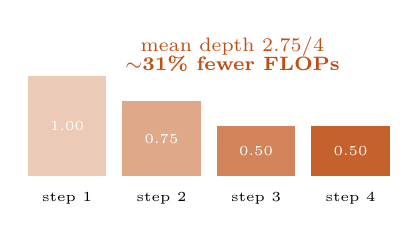
\begin{tikzpicture}[node distance=1mm]
  \foreach \x/\w/\f in {0/4/1.00, 1/3/0.75, 2/2/0.50, 3/2/0.50}{
    \fill[accentB!\the\numexpr30+20*\x\relax] (\x*1.2,0) rectangle ++(1,\w*0.32);
    \node[font=\tiny] at (\x*1.2+0.5,-0.28) {step \the\numexpr\x+1\relax};
    \node[font=\tiny, text=white] at (\x*1.2+0.5,\w*0.16) {\f};
  }
  \node[font=\scriptsize, text=accentB, align=center] at (2.6,1.55)
     {mean depth $2.75/4$\\[-1pt]\comp{$\sim$31\% fewer FLOPs}};
\end{tikzpicture}}
\vspace{1mm}

\begin{block}{\footnotesize Verdicts (multi-seed, statistical)}
\scriptsize
\comp{$+$} Adaptive depth: \comp{$\sim$31\% compute saved} at matched accuracy \& params ($p\!<\!0.001$).\\[2pt]
\bad{$-$} Biological prior vs random-graph: $\Delta$F1 $=\!+0.28$, $p\!=\!0.871$, \bad{0/10 significant}.\\[2pt]
\bad{$-$} Adaptive vs vanilla accuracy \& calibration: \bad{no consistent gain}.
\end{block}
\end{columns}
\end{frame}

% ======================= SLIDE 3: biology + directions =====================
\begin{frame}{Biologically meaningful token reduction --- and where to push next}
\begin{columns}[T]
\column{0.46\textwidth}
\centering
\resizebox{\linewidth}{!}{%
\begin{tikzpicture}[node distance=5mm]
  \node[stage, fill=panelA] (t1) {{\textcolor{accentA}{\faTag}}\\[1pt]\textbf{marker token}};
  \node[stage, below=of t1, fill=panelA] (t2) {{\textcolor{accentA}{\faDna}}\\[1pt]\textbf{gene program}};
  \node[stage, below=of t2, fill=panelA] (t3) {{\textcolor{accentA}{\faSitemap}}\\[1pt]\textbf{pathway}};
  \node[stage, right=16mm of t2, fill=panelB, text width=24mm] (imp)
       {{\textcolor{accentB}{\faSortAmountDown}}\\[1pt]\textbf{survival depth}\\[1pt]{\tiny\textcolor{subcap}{= importance rank}}};
  \draw[bioflow] (t1) -- (imp);
  \draw[bioflow] (t2) -- (imp);
  \draw[bioflow] (t3) -- (imp);
\end{tikzpicture}}
\vspace{1mm}\\
{\scriptsize Each token $\approx$ a learned \good{signature / gene program} --- a deployable \good{marker panel}, not a black box. A token's \good{recursion depth} is a compute-based \good{importance score}.}

\column{0.54\textwidth}
\textbf{\footnotesize Negatives $\Rightarrow$ directions}
\begin{itemize}\footnotesize
  \item \good{Stronger injection:} prior is an additive, annealed-away bias $\to$ use \good{FiLM/gating} so centrality \emph{modulates} routing per cell.
  \item \good{Better graph:} swap co-expression centrality for \good{directed GRNs / perturbation graphs} (causal, not correlational).
  \item \good{Right granularity:} route \good{pathway tokens} $\Rightarrow$ "depth per pathway" = compute a biological process needs.
  \item \good{Validate:} check survival-depth rankings against \good{known lineage / disease markers}.
\end{itemize}
\vspace{1mm}
{\footnotesize\good{Take-away:} token reduction is the biologically meaningful lever that \emph{works}; the bio prior is a promising direction, reported honestly.}
\end{columns}
\end{frame}

% ============ SLIDE 4: why the LEARNED data-driven graph works ==============
\begin{frame}{Why a \emph{learned} graph beats a fixed biological one}
\begin{columns}[T]
\column{0.52\textwidth}
\textbf{\footnotesize The router smooths expression along a gene graph $A$:}
\[
   \tilde{x} \;=\; (1-\lambda)\,x \;+\; \lambda\, A\,x .
\]
\textbf{\footnotesize Fixed $A$ (co-expression / Reactome):}
\begin{itemize}\footnotesize
  \item label-free $\Rightarrow \partial \mathcal{L}/\partial A = 0$ (edges never learn);
  \item annealed $\Rightarrow$ converged model $\equiv$ \texttt{none};
  \item a degree-matched \emph{shuffle} gives the same generic smoothing:
        \bad{$\mathbb{E}[\text{bio}]=\mathbb{E}[\text{random}]$} \; (FACT B).
\end{itemize}
\vspace{1mm}
\textbf{\footnotesize Learned $A=\tilde{E}\tilde{E}^{\!\top}$ (rank $r$, embedding $E$):}
\[
  \tilde{x} = (1-\lambda)x + \lambda\,(x\tilde{E})\tilde{E}^{\!\top},
  \qquad \tfrac{\partial \mathcal{L}}{\partial E}\neq 0 .
\]
\good{Edges are chosen to cut the loss.} Low rank $\Rightarrow$ $r$ latent
\good{gene programs}; propagation denoises each gene toward its program's consensus,
and \good{supervision makes those programs discriminative} (not variance-maximal like
PCA, not fixed like Reactome).

\column{0.48\textwidth}
\centering
\textbf{\footnotesize One patient, two co-varying markers}
\begin{block}{}\footnotesize
Genes $g_1,g_2$: weak, \emph{noisy}, but co-vary with the label.
\smallskip

\good{Learned graph} learns $\tilde{E}_{g_1}\!\approx\!\tilde{E}_{g_2}$ (same program):
\[
  \tilde{x}_{g_1}\approx\tfrac12\big(x_{g_1}+x_{g_2}\big)
\]
independent noise averages down (\good{$\times\sqrt{2}$ SNR}), shared signal kept
$\Rightarrow$ a \good{cleaner marker token}.
\smallskip

\bad{Random / fixed graph} links $g_1$ to \emph{unrelated} genes $\Rightarrow$ averages
\emph{in} noise $\Rightarrow$ over-smooths, no SNR gain.
\end{block}
\vspace{1mm}
{\footnotesize\good{On data (P-NET, 10 seeds):} learned $-$ none $=\mathbf{+1.9}$ F1
(\good{$p{=}.043$}); \good{$+5.7$} on prostate. Beats co-expression, Reactome
\emph{and} random --- the first mechanism that does.}
\end{columns}
\end{frame}

\end{document}
